%%%%%%%%%%%%%%%%%%%%%%%%%%%%%%%%%%%%%%%%%
% a0poster Portrait Poster
% LaTeX Template
% Version 1.0 (22/06/13)
%
% The a0poster class was created by:
% Gerlinde Kettl and Matthias Weiser (tex@kettl.de)
% 
% This template has been downloaded from:
% http://www.LaTeXTemplates.com
%
% License:
% CC BY-NC-SA 3.0 (http://creativecommons.org/licenses/by-nc-sa/3.0/)
%
%%%%%%%%%%%%%%%%%%%%%%%%%%%%%%%%%%%%%%%%%

%----------------------------------------------------------------------------------------
%	PACKAGES AND OTHER DOCUMENT CONFIGURATIONS
%----------------------------------------------------------------------------------------

\documentclass[a0,portrait]{poster}

\usepackage{multicol} % This is so we can have multiple columns of text side-by-side
\columnsep=100pt % This is the amount of white space between the columns in the poster
\columnseprule=3pt % This is the thickness of the black line between the columns in the poster

\usepackage[svgnames]{xcolor} % Specify colors by their 'svgnames', for a full list of all colors available see here: http://www.latextemplates.com/svgnames-colors

\usepackage{times} % Use the times font
%\usepackage{palatino} % Uncomment to use the Palatino font

\usepackage{graphicx} % Required for including images
\usepackage{booktabs} % Top and bottom rules for table
\usepackage[font=small,labelfont=bf]{caption} % Required for specifying captions to tables and figures
\usepackage{amsfonts, amsmath, amsthm, amssymb} % For math fonts, symbols and environments
\usepackage{wrapfig} % Allows wrapping text around tables and figures

\begin{document}

%----------------------------------------------------------------------------------------
%	POSTER HEADER 
%----------------------------------------------------------------------------------------

% The header is divided into two boxes:
% The first is 75% wide and houses the title, subtitle, names, university/organization and contact information
% The second is 25% wide and houses a logo for your university/organization or a photo of you
% The widths of these boxes can be easily edited to accommodate your content as you see fit

\begin{minipage}[b]{0.6\linewidth}
\veryHuge \color{NavyBlue} \textbf{NDNCERT in Identity Manager} \color{Black}\\ % Title
\Huge\textit{A trial to implement an identity manage using NDNCERT in Named Data Networking(NDN)}\\[2cm] % Subtitle
\Large \textbf{Yuyang(Peter) Rong, Arthi Padmanabhan, Lixia Zhang \footnotemark}\\[0.5cm] % Author(s)
\Large ShanghaiTech / UCLA \\ [0.4cm] % University/organization
\Large \texttt{PeterRong96@gmail.com} --- +1 (310) 307 9952\\
\end{minipage}
\footnotetext{	
	We also want to thank the following people for their help:
	Lixia Zhang, Arthi Padmanabhan, Zhiyi Zhang and Alex Afanasyev. They helped a lot when developing this application. 
	Ren Sun and CSST for providing such great opportunity.
}
%
\begin{minipage}[b]{0.4\linewidth}
	
\includegraphics[width=\linewidth]{figures/logo.png}\\
\end{minipage}

\vspace{0.7cm} % A bit of extra whitespace between the header and poster content

%----------------------------------------------------------------------------------------

\begin{multicols}{2} % This is how many columns your poster will be broken into, a portrait poster is generally split into 2 columns

%----------------------------------------------------------------------------------------
%	ABSTRACT
%----------------------------------------------------------------------------------------

%\color{Navy} % Navy color for the abstract

%\begin{abstract}

%	Security and privacy in networking are gaining more and more attention nowadays. 
%	NDN is a newly proposed architecture that has shown great potential in security. 
%	In NDN, each packet has to be signed and thus is secured. 
%	In this work, we use NDNCERT, a certificate manager, to request and manage certificates that can be used to sign data packets. 
%	We would install this manager in cell phones and thus allow other applications like NDNFit to gain certificate through this manager. 

%\end{abstract}

%----------------------------------------------------------------------------------------
%	INTRODUCTION
%----------------------------------------------------------------------------------------

\color{SaddleBrown} % SaddleBrown color for the introduction
\section*{Problem}
	Security and privacy in networking are gaining more and more attention nowadays. 
	NDN is a newly proposed architecture that has shown great potential in security. 
	In NDN, each packet has to be signed and thus is secured. 
	But in applications like NDNFit, signing entity cannot be trusted.
	In this work, we would be using NDNCERT to get a certificate for appliations in NDNFit.
	These issued certificates make them trustworthy.
%----------------------------------------------------------------------------------------
%	OBJECTIVES
%----------------------------------------------------------------------------------------

\color{DarkSlateGray} % DarkSlateGray color for the rest of the content

\section*{Main Objectives}

\begin{enumerate}
\item Use NDNCERT to write identity manager;
\item Explore NDN development on Android and provide experience for other apps;
\item Provide an identity manager to update NDNFit.
\end{enumerate}

%----------------------------------------------------------------------------------------
%	MATERIALS AND METHODS
%----------------------------------------------------------------------------------------

\section*{Packages}

\begin{minipage}[b]{0.3\linewidth}
\subsection*{NDN\cite{zhang2014named}}
\par
	\begin{itemize}
		\item Interest \& Data;
		\item Both have to be signed and thus verifiable.
	\end{itemize}

\subsection*{NDNFit\cite{zhang2018ndnfit}}
\par
	\begin{itemize}
		\item A set of applications runs on NDN;
		\item DSU, DVU, DPU \& Identity manager
		\item Different namespaces for each application and user
		\item Identity manager manages all the identities.
	\end{itemize}
\par
\end{minipage}
\begin{minipage}[b]{0.65\linewidth}
	\includegraphics[width=\linewidth]{figures/NDNfit.png}
\end{minipage}


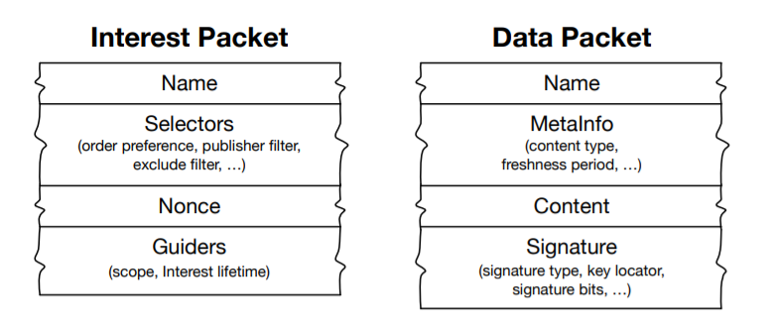
\includegraphics[width=\linewidth]{figures/packet.png}

\subsection*{NDN Certificate management protocol(NDNCERT)\cite{zhang2017ndncert}}
\begin{itemize}
	\item A protocol that allows auto certificate managerment;
	\item Identity will request certificate from Certificate Authority(CA);
	\item NDNCERT will be placed in identity manager;
	\item Once the certificate is acquired, it will be used to manage that namespace.
\end{itemize}


%------------------------------------------------
%\subsection*{Android \& Java Native Interface(JNI)}
%\par 
%	Applications like NDNFit require mobile clients. 
%	In our case, we preferred Android over Apple, as Android are easier to develop and test.
%	What's more, in the long run Android can be rooted to support NDN, yet Apple can't.
%	Android has to be developed using Java, yet NDNCERT and NDN are written in c++. 
%	Whether or not to use JNI has been a problem. 
%	JNI provides native access to non-Java languages, allowing us to call c/c++ functions using Java. 
%	In our first implementation we didn't use Java, instead we rewrote NDNCERT using Java. The benefits includes:
%	\begin{itemize}
%		\item No overheads for calling JNI.
%		\item Easier to program/debug than JNI.
%	\end{itemize}
%\par
%	However, soon we realized that they are downsizes too:
%	\begin{itemize}
%		\item Code base may be too hard to maintain. Same feature has to be implemented/ debugged twice.
%	\end{itemize}
%\par
%	We implemented both and compared the process and the difficulty of developing.

%----------------------------------------------------------------------------------------
%	RESULTS 
%----------------------------------------------------------------------------------------

\section*{Result}
\begin{itemize}
	\item Our identity manager has a new UI
	\item Following the steps the user can create a new certificate
	\item At the first time NDNFit is started, a certificate will be distributed by identity manager
\end{itemize}

\begin{minipage}[b]{0.57\linewidth}
	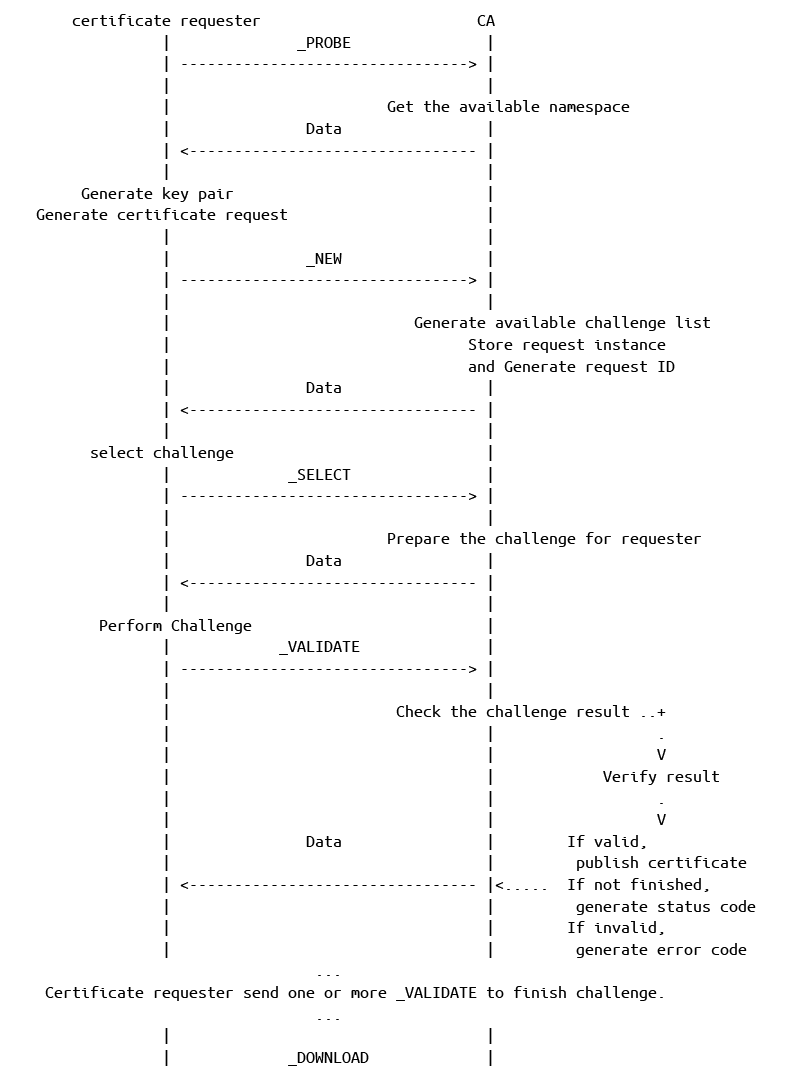
\includegraphics[width=\linewidth]{figures/protocol.png}
\end{minipage}
\begin{minipage}[b]{0.43\linewidth}
	\centering
	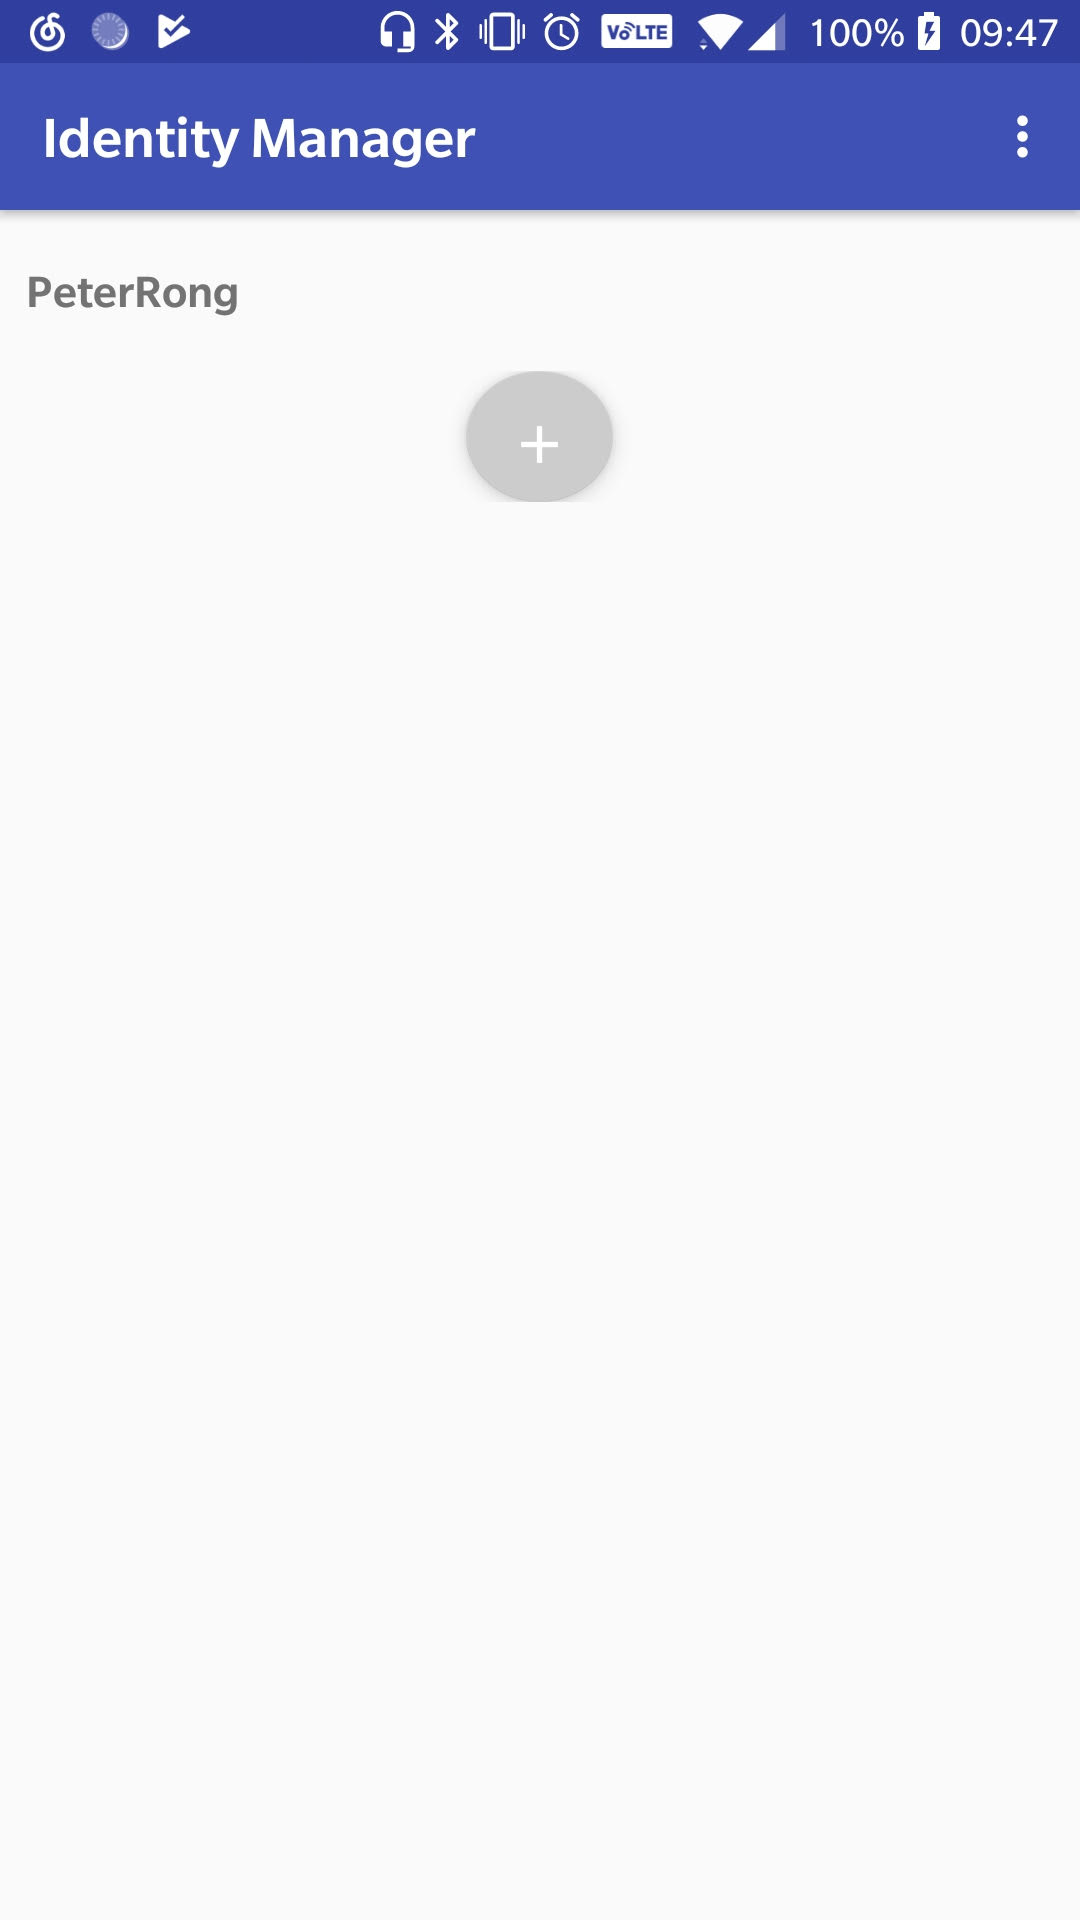
\includegraphics[width=\linewidth]{figures/main-activity.jpg}
\end{minipage}

\begin{center}
	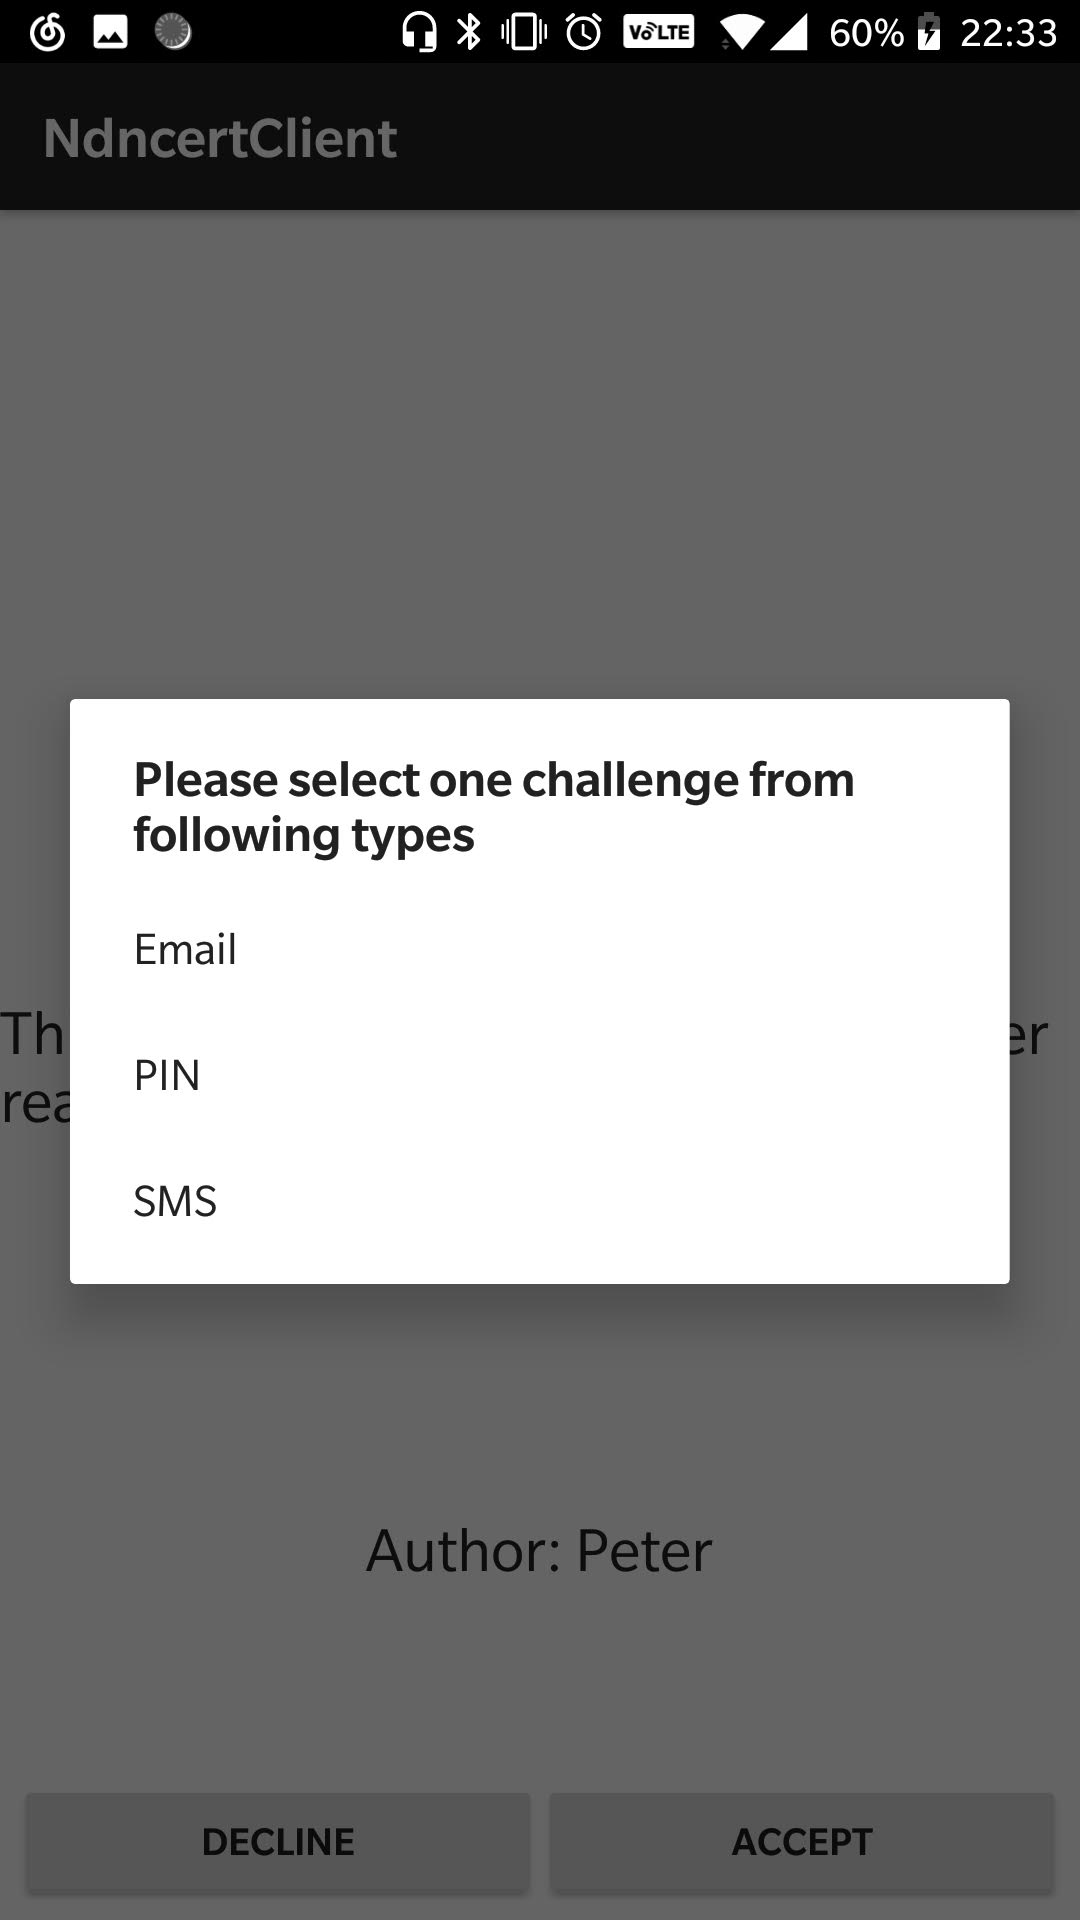
\includegraphics[width=0.27\linewidth]{figures/select.jpg}
	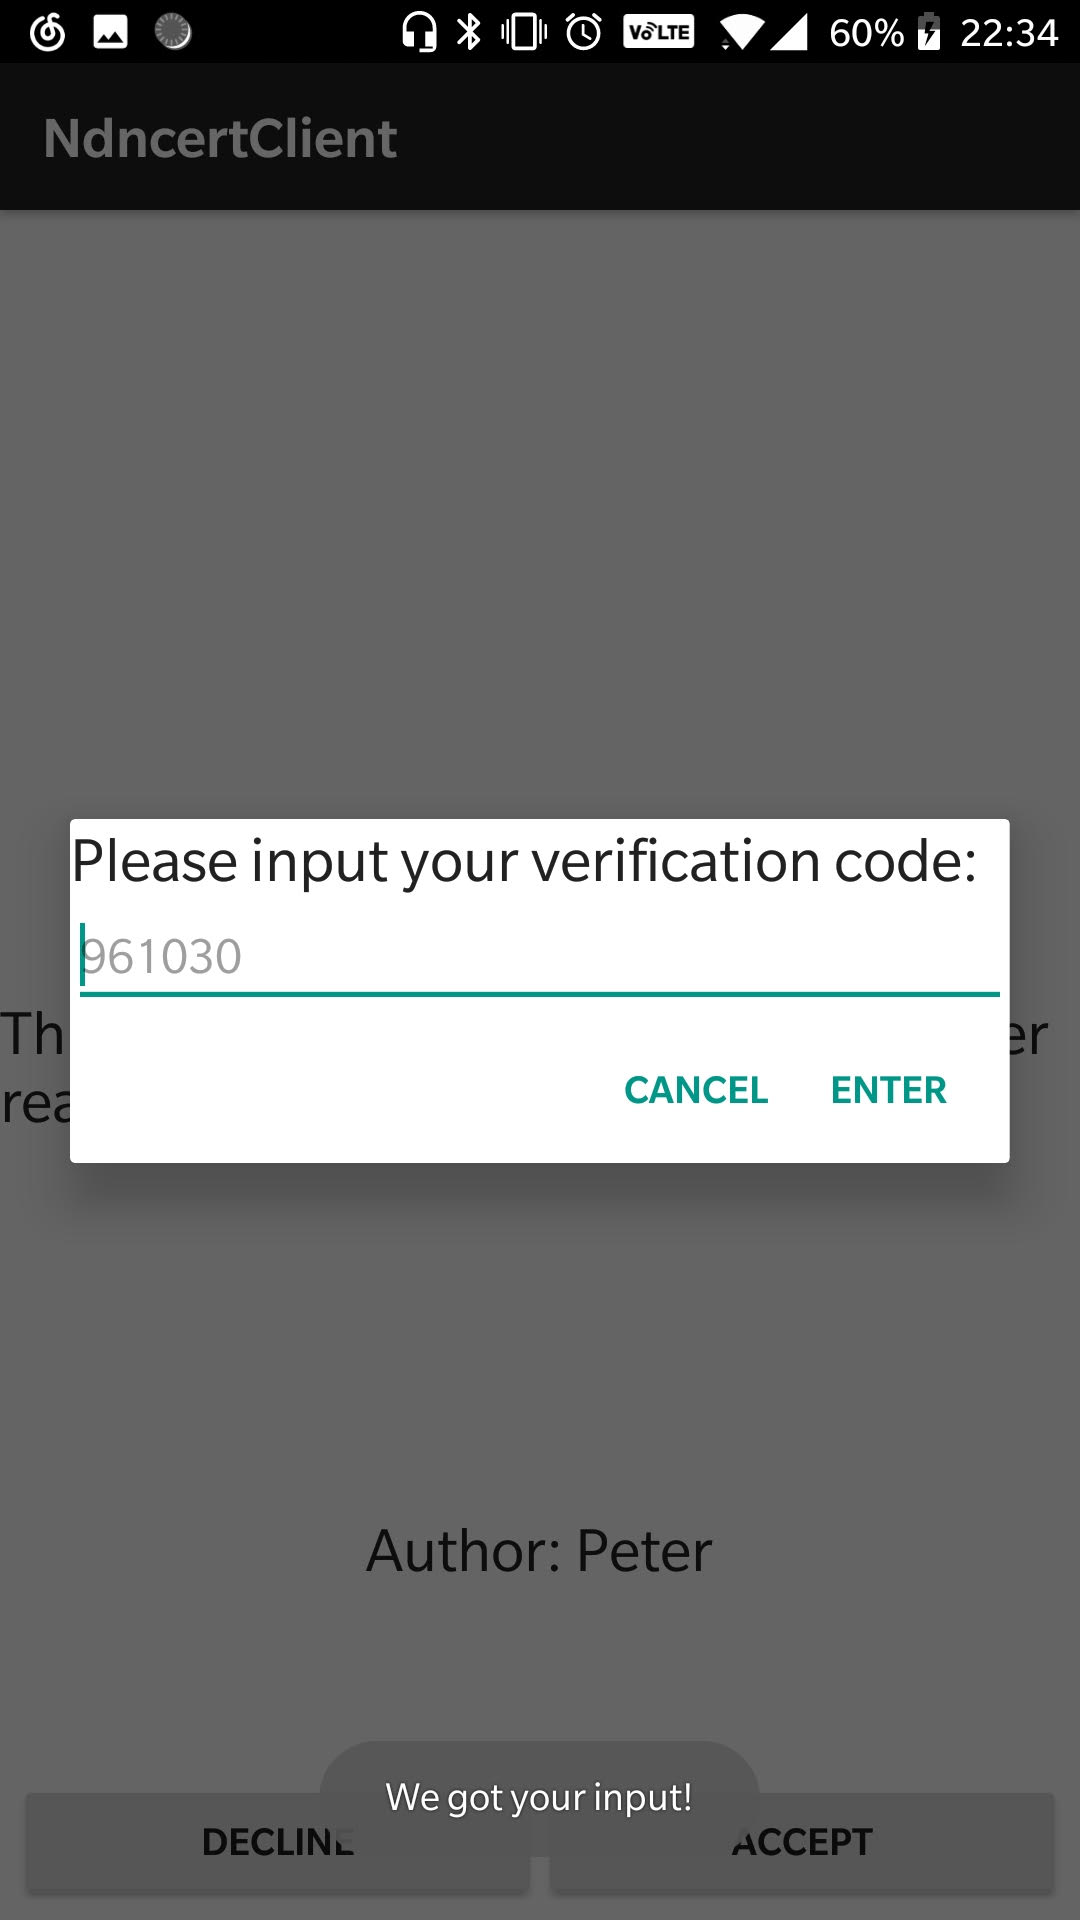
\includegraphics[width=0.27\linewidth]{figures/validate.jpg}
	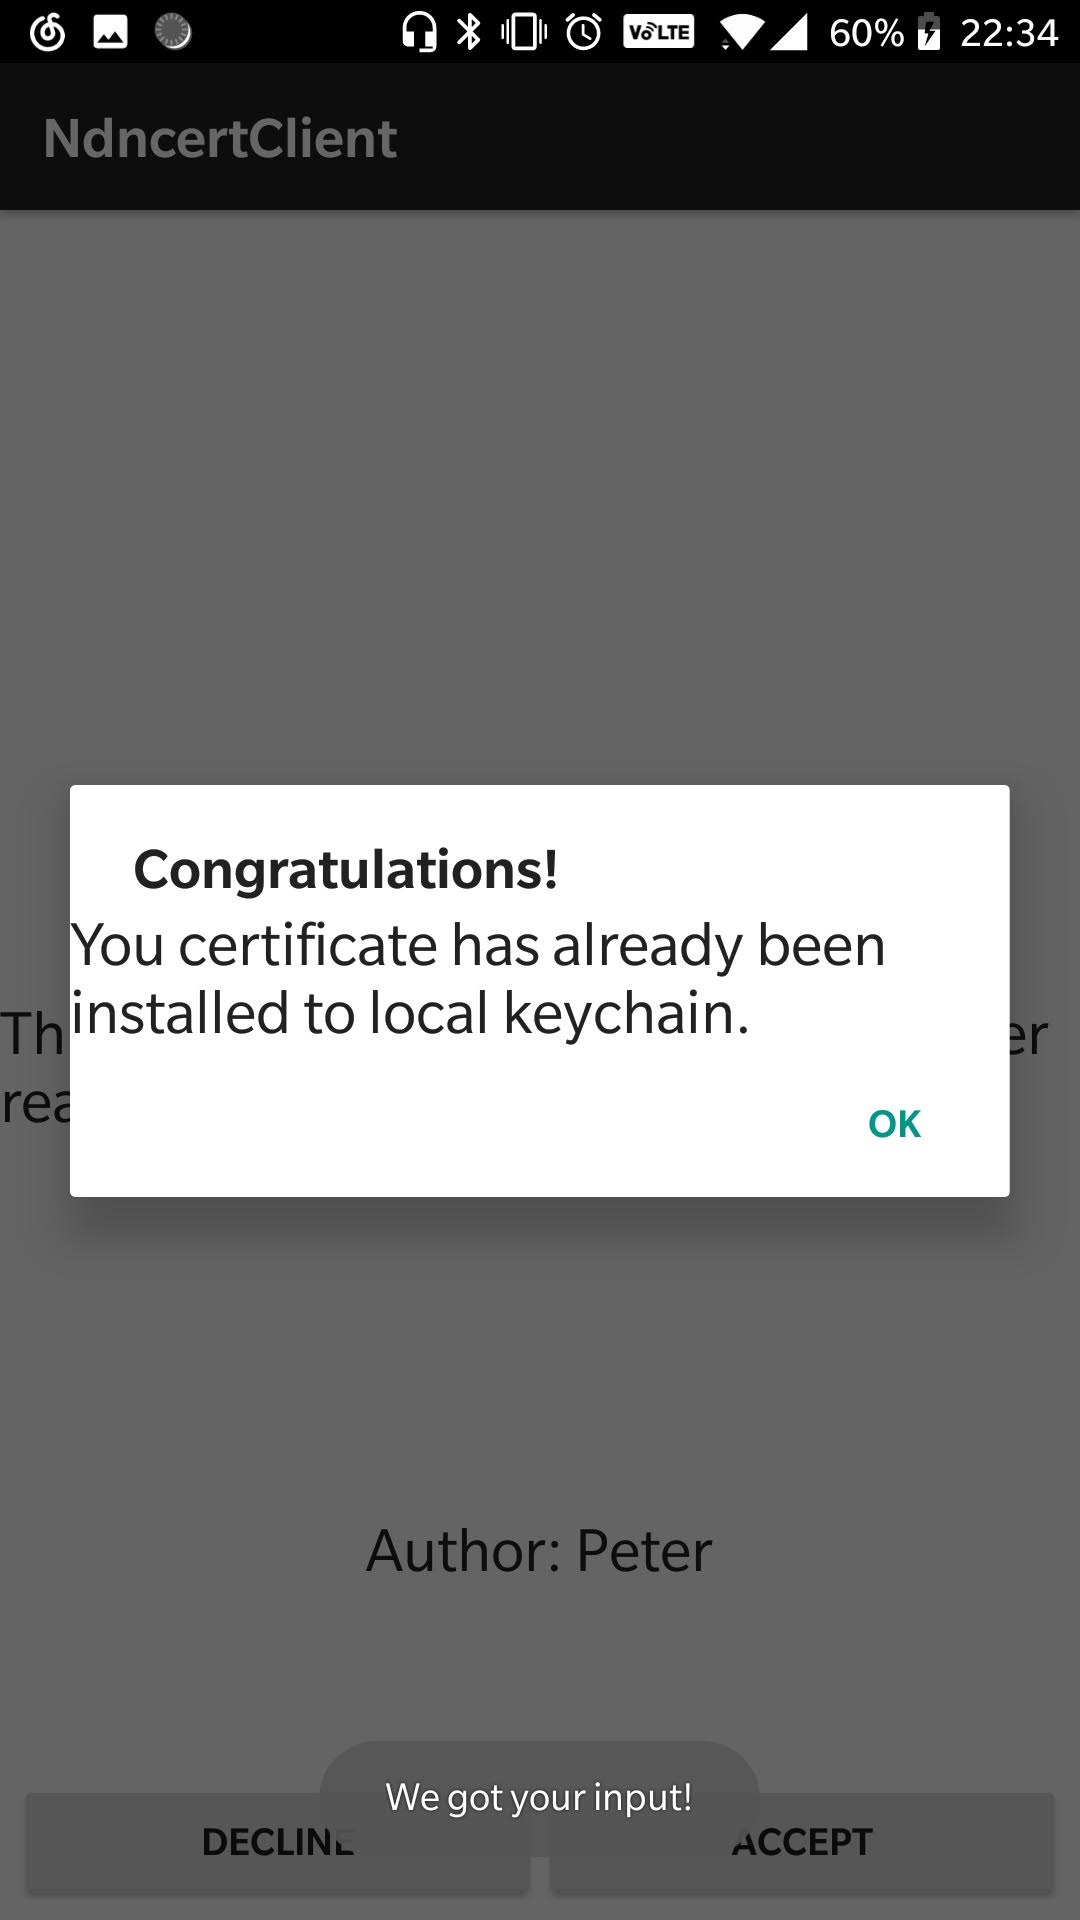
\includegraphics[width=0.27\linewidth]{figures/download.jpg}
\end{center}
%----------------------------------------------------------------------------------------
%	CONCLUSIONS
%----------------------------------------------------------------------------------------

%\color{SaddleBrown} % SaddleBrown color for the conclusions to make them stand out

%\section*{Conclusions}

%\color{DarkSlateGray} % Set the color back to DarkSlateGray for the rest of the content

%----------------------------------------------------------------------------------------
%	FORTHCOMING RESEARCH
%----------------------------------------------------------------------------------------

\section*{Future Work}

\par 
	Identity manager is about to be functional, and there are more details that can be added, including:
	\begin{itemize}
		\item identity deleting, 
		\item collision handling when identities have same name,
		\item certificate distribute when requested by other app.
	\end{itemize} 

%----------------------------------------------------------------------------------------
%	REFERENCES
%----------------------------------------------------------------------------------------

\nocite{*} % Print all references regardless of whether they were cited in the poster or not
\bibliographystyle{plain} % Plain referencing style
\bibliography{reference}
%----------------------------------------------------------------------------------------
%	ACKNOWLEDGEMENTS
%----------------------------------------------------------------------------------------

%\section*{Acknowledgments}

%\par
%	\footnotesize{We would like to thank the following people for their help:}
%	\footnotesize{
%		Lixia Zhang, Arthi Padmanabhan, Zhiyi Zhang and Alex Afanasyev. 
%		Ren Sun and CSST for providing such great opportunity.
%	}
%----------------------------------------------------------------------------------------

\end{multicols}
\end{document}